% =======================================================================================================
\section{Implementação}
\label{sec:impl}

O relatório usa duas implementações independentes da mesma rede: a do scikit-learn, madura e
otimizada, e uma implementação manual em NumPy, escrita para tornar a matemática visível. A
concordância entre as duas é, ela mesma, uma forma de validação.

\subsection{Organização do código}

O script \texttt{mlp\_iris.py} é organizado em etapas numeradas, na ordem em que aparecem no
relatório:

\begin{enumerate}
	\item leitura dos dados e análise exploratória;
	\item estudo de arquiteturas;
	\item estudo de funções de ativação;
	\item estudo da regularização $L_2$;
	\item estudo da taxa de aprendizado;
	\item curvas de treinamento e de aprendizado;
	\item divisão treino/teste e métricas finais;
	\item fronteiras de decisão e importância de atributos;
	\item visualização dos pesos;
	\item verificação numérica do gradiente e implementação em NumPy;
	\item comparação com modelos de referência e testes estatísticos.
\end{enumerate}

Cada etapa grava seus resultados em arquivo: métricas em CSV, figuras em PNG e tabelas em LaTeX.
Isso permite que o documento incorpore as tabelas diretamente, sem transcrição manual.

\subsection{O pipeline do scikit-learn}

O modelo é definido como um \texttt{Pipeline} de dois passos: padronização e MLP. A vantagem não é
estética: dentro da validação cruzada, o \texttt{Pipeline} garante que o \texttt{StandardScaler}
seja ajustado apenas na dobra de treino, eliminando o vazamento discutido no
\secao{sec:metodo}.

\begin{lstlisting}[caption={Definição do modelo principal (extrato de \texttt{mlp\_iris.py}).},label={lst:pipeline}]
def mlp(hidden=(16, 8), ativacao="relu", alpha=1e-3, semente=42,
        solver="adam", lr=1e-3, max_iter=3000, early_stopping=False):
    """Pipeline padronizacao + MLP (ajustado dentro de cada dobra)."""
    return make_pipeline(
        StandardScaler(),
        MLPClassifier(hidden_layer_sizes=hidden, activation=ativacao, alpha=alpha,
                      solver=solver, learning_rate_init=lr, max_iter=max_iter,
                      early_stopping=early_stopping, validation_fraction=0.15,
                      n_iter_no_change=40, random_state=semente),
    )

MLP_PRINCIPAL = dict(hidden=(16,), ativacao="tanh", alpha=1e-2)
\end{lstlisting}

Os hiperparâmetros têm o seguinte significado:

\begin{itemize}
	\item \texttt{hidden\_layer\_sizes}: tupla com o número de neurônios de cada camada oculta;
	\item \texttt{activation}: função de ativação das camadas ocultas;
	\item \texttt{alpha}: coeficiente $\lambda$ da penalidade $L_2$;
	\item \texttt{solver}: \texttt{adam}, \texttt{sgd} ou \texttt{lbfgs};
	\item \texttt{learning\_rate\_init}: taxa de aprendizado inicial $\eta_0$;
	\item \texttt{max\_iter}: número máximo de épocas;
	\item \texttt{early\_stopping}: ativa a parada antecipada com \texttt{validation\_fraction}
	      dos dados de treino;
	\item \texttt{n\_iter\_no\_change}: paciência, em épocas, antes de parar.
\end{itemize}

\subsection{Implementação manual em NumPy}

A implementação manual segue exatamente as equações do \secao{sec:mlp}. A classe
\texttt{MLPNumPy} guarda $\bW^{(1)},\bb^{(1)},\bW^{(2)},\bb^{(2)}$ e implementa a propagação
direta, a perda com regularização, a retropropagação e o passo de Adam.

\begin{lstlisting}[caption={Núcleo da implementação manual: propagação direta e retropropagação.},label={lst:numpy}]
def forward(self, X):
    z1 = X @ self.W1 + self.b1        # (m, h)  pre-ativacao da oculta
    a1 = self._f(z1)                  # (m, h)  ativacao da oculta
    z2 = a1 @ self.W2 + self.b2       # (m, C)  escores da saida
    return z1, a1, z2, _softmax(z2)   # (m, C)  probabilidades

def perda(self, X, y):
    _, _, _, p = self.forward(X)
    Y = _onehot(y)
    ce = -np.mean(np.sum(Y * np.log(p + 1e-12), axis=1))
    reg = 0.5 * self.alpha * (np.sum(self.W1 ** 2) + np.sum(self.W2 ** 2))
    return ce + reg

def backward(self, X, y):
    m = len(y)
    z1, a1, _, p = self.forward(X)
    Y = _onehot(y)
    d2 = (p - Y) / m                        # Delta^(2) = (P - Y)/m
    gW2 = a1.T @ d2 + self.alpha * self.W2  # gradiente + L2
    gb2 = d2.sum(0)
    d1 = (d2 @ self.W2.T) * self._df(z1)    # Delta^(1)
    gW1 = X.T @ d1 + self.alpha * self.W1
    gb1 = d1.sum(0)
    return {"W1": gW1, "b1": gb1, "W2": gW2, "b2": gb2}
\end{lstlisting}

O laço de treinamento aplica Adam, com as equações \equacao{eq:adam-m}--\equacao{eq:adam-upd},
a minilotes de 16 amostras embaralhadas a cada época:

\begin{lstlisting}[caption={Laço de treinamento com Adam (extrato).},label={lst:adam}]
for ep in range(epocas):
    ordem = rng.permutation(len(y))
    for i in range(0, len(y), lote):
        idx = ordem[i:i + lote]
        g = self.backward(X[idx], y[idx])
        t += 1
        for k in params:
            m[k] = b1 * m[k] + (1 - b1) * g[k]
            v[k] = b2 * v[k] + (1 - b2) * g[k] ** 2
            mh = m[k] / (1 - b1 ** t)       # correcao de vies
            vh = v[k] / (1 - b2 ** t)
            params[k] -= lr * mh / (np.sqrt(vh) + eps)
\end{lstlisting}

A \figura{fig:implementacao} compara as duas implementações. Com a mesma arquitetura
(8 neurônios ocultos), a implementação manual e a do scikit-learn alcançam exatamente a mesma
acurácia no teste (\accNumpy{} e \accSklearn{}), e a curva de perda da versão manual decresce de
forma suave, com as oscilações típicas do treinamento por minilotes.

\begin{figure}[htbp]
	\centering
	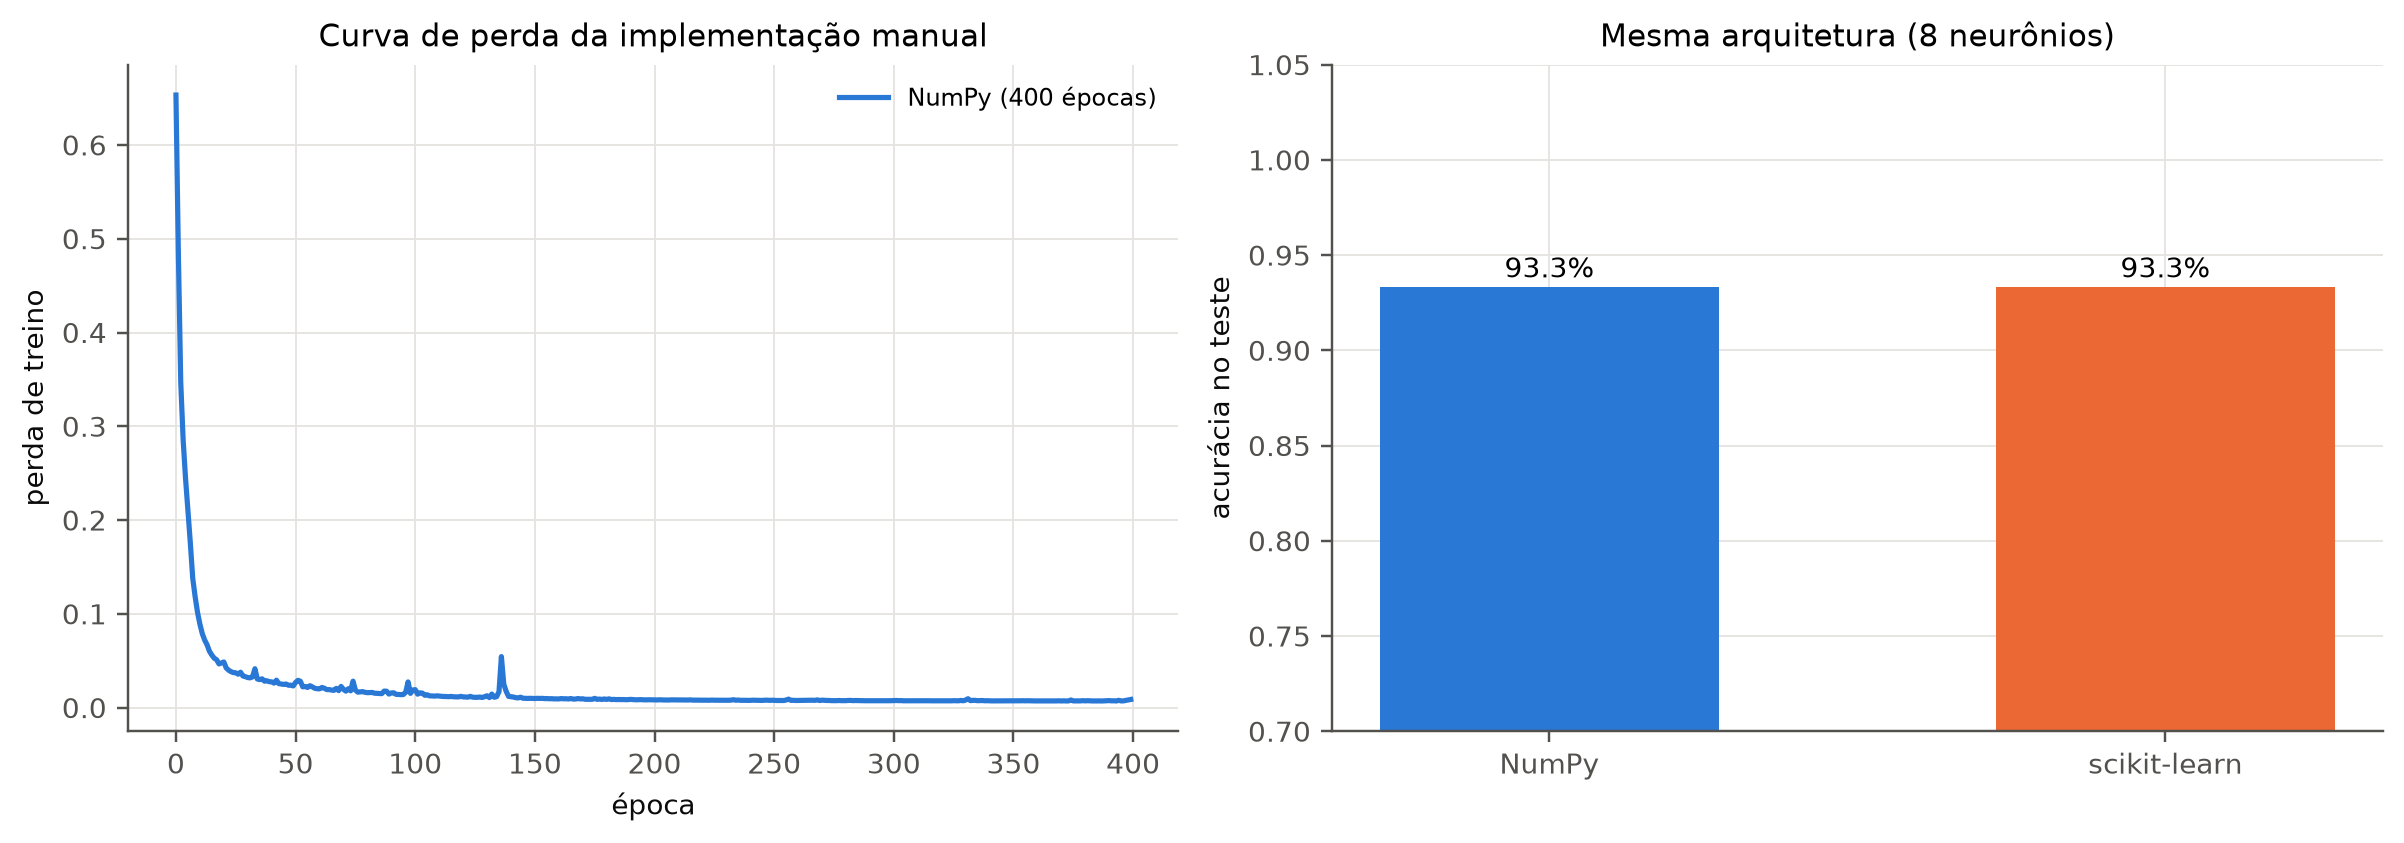
\includegraphics[width=\textwidth]{fig_implementacao.png}
	\caption{À esquerda, curva de perda da implementação manual em NumPy (400 épocas, Adam,
	minilotes de 16). À direita, acurácia no conjunto de teste das duas implementações com a mesma
	arquitetura.}
	\label{fig:implementacao}
\end{figure}

\subsection{Verificação numérica do gradiente}

A retropropagação é a parte mais sujeita a erro de implementação, porque envolve transposições e
produtos elemento a elemento que ``quase'' funcionam quando estão errados. O teste padrão compara
o gradiente analítico com uma aproximação por diferenças centrais, \equacao{eq:gradcheck}, em uma
rede pequena ($4$--$5$--$3$, ativação \emph{tanh}) e em um subconjunto de amostras.

O resultado está na \figura{fig:gradiente}. Os pontos caem praticamente sobre a diagonal
identidade, e o erro relativo máximo é \erroGrad{} --- ordens de grandeza abaixo do limiar de
$10^{-4}$ usado na prática. Isso confirma tanto a derivação quanto o código: se houvesse um erro
de sinal, de transposição ou de normalização, o erro relativo seria da ordem de $10^{-1}$ ou
maior.

\begin{figure}[htbp]
	\centering
	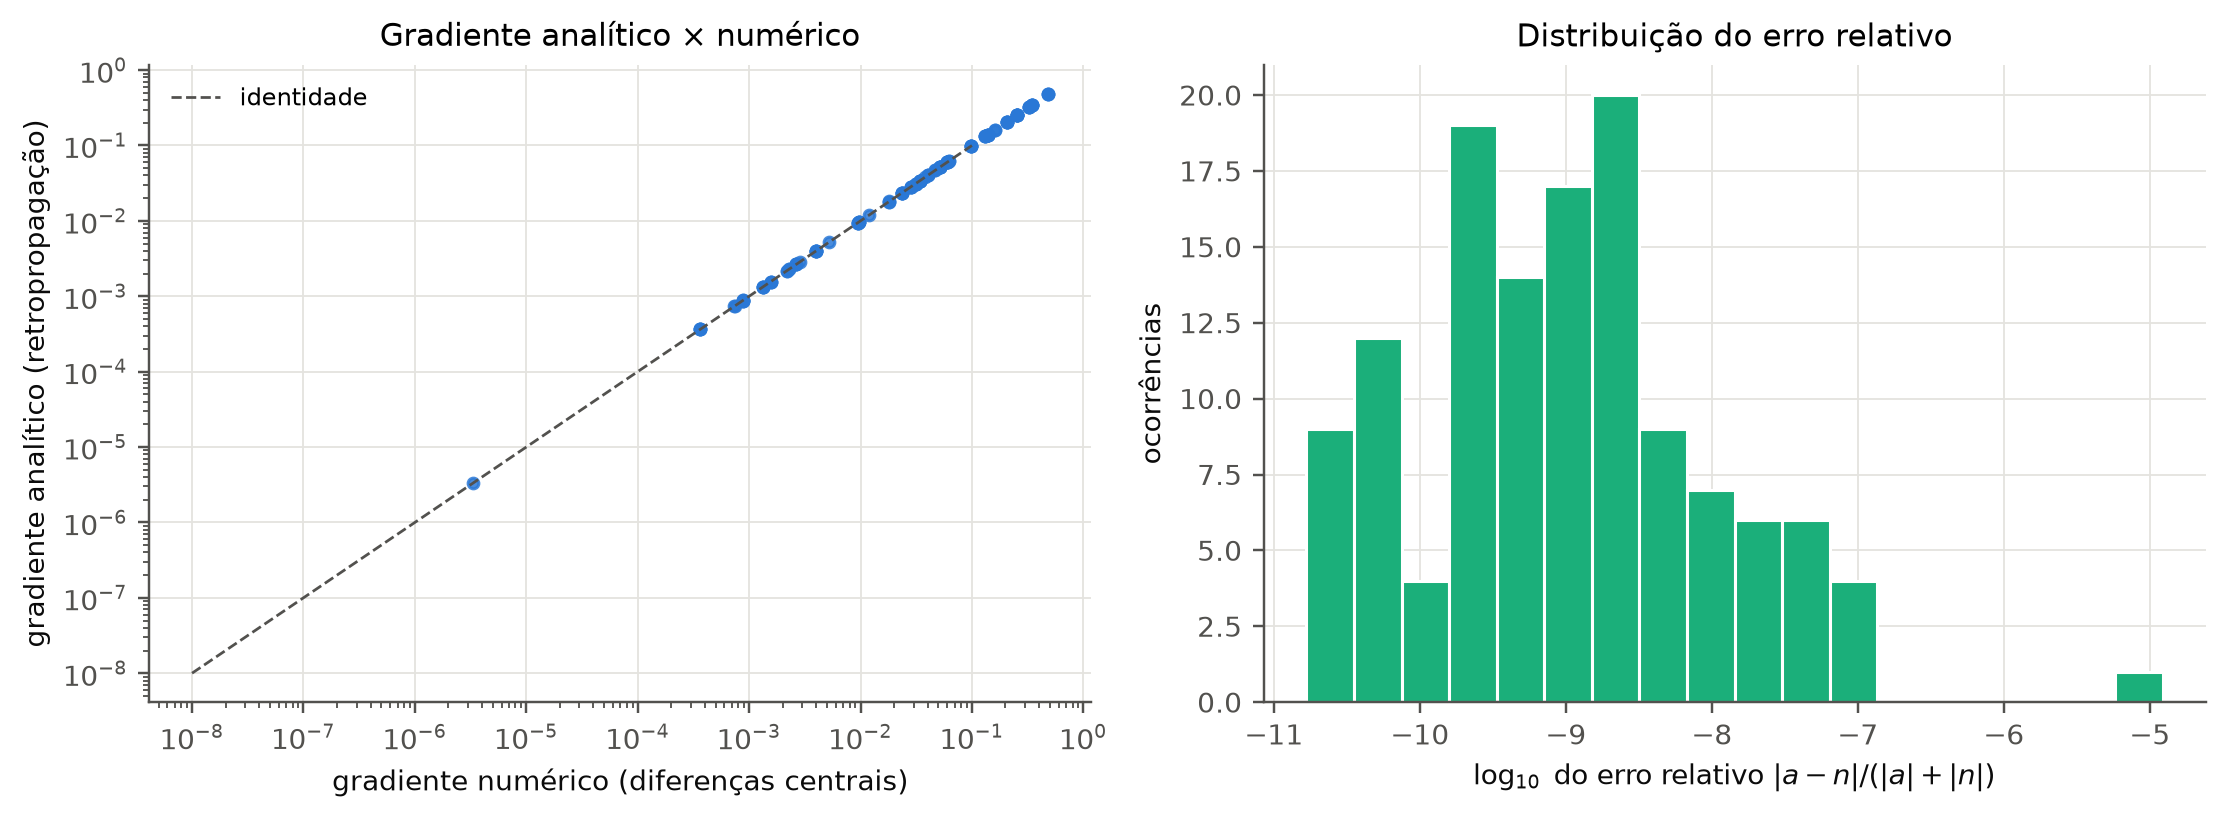
\includegraphics[width=\textwidth]{fig_gradiente.png}
	\caption{Verificação do gradiente. À esquerda, gradiente analítico contra numérico para os
	parâmetros amostrados; a linha tracejada é a identidade. À direita, distribuição do erro
	relativo, em escala logarítmica.}
	\label{fig:gradiente}
\end{figure}

\begin{table}[htbp]
	\centering
	\caption{Erro relativo da checagem de gradiente por matriz de parâmetros.}
	\label{tab:gradiente}
	% gerado automaticamente por mlp_iris.py - nao editar

\begin{tabular}{lrrr}
\toprule
\textbf{parâmetro} & \textbf{amostras} & \textbf{erro máximo} & \textbf{erro médio} \\
\midrule
W1 & 60 & $6{,}8\times10^{-8}$ & $1{,}2\times10^{-8}$ \\
b1 & 5 & $1{,}2\times10^{-5}$ & $2{,}5\times10^{-6}$ \\
W2 & 60 & $4{,}2\times10^{-9}$ & $1{,}3\times10^{-9}$ \\
b2 & 3 & $7{,}4\times10^{-9}$ & $3{,}2\times10^{-9}$ \\
\bottomrule
\end{tabular}

\end{table}

\subsection{Detalhes de engenharia}

Três decisões de implementação merecem registro, porque afetam a reprodutibilidade.

\paragraph{Semente única.} A semente é propagada para a divisão dos dados, para a inicialização
dos pesos e para as partições da validação cruzada. Sem isso, duas execuções do mesmo código
produziriam resultados diferentes e nenhuma conclusão seria verificável.

\paragraph{Isolamento de threads.} Bibliotecas numéricas usam múltiplas threads por padrão. Com
150 amostras, o custo de coordenar threads é maior que o ganho, e a variação de tempo entre
execuções atrapalha a comparação. O script fixa as variáveis de ambiente
\texttt{OMP\_NUM\_THREADS}, \texttt{OPENBLAS\_NUM\_THREADS} e \texttt{MKL\_NUM\_THREADS} em $1$.

\paragraph{Formato dos números.} Os arquivos de tabela usam vírgula decimal e protegem os
algarismos com chaves (\texttt{0\{,\}968}), para que o mesmo número funcione em modo texto e em
modo matemático no \LaTeX{}. As figuras usam a vírgula diretamente, porque são rasterizadas.
